\documentclass[../libro.tex]{subfiles}

% I use this package to make figures.
\usepackage{tikz}
\usetikzlibrary{calc,matrix}

\begin{document}

\ifSubfilesClassLoaded{\mainmatter\chapter{行列式}\clearpage}{}

\section{阵}

虽然, 理论地, 我可不用阵 (矩形数表)
直接讲行列式,
但为方便, 我决定先介绍阵的基础.
相应地, 行列式会被定义为方阵
(正方形数表)
的一个属性.

\begin{definition}[阵]
    设 \(m\), \(n\) 是正整数.
    我们说,
    由 \(mn\) 个文字作成的 \(m \times n\) 矩形文字表
    (这里, ``文字'' 一般是数,
    如整数、可比数 (\angla{rational numbers})、实数;
    当然, ``文字'' 也能是跟数有关, 但不是数的对象,
    如整式、分式)
    \begin{align*}
        A =
        \begin{bmatrix}
            [A]_{1,1} & [A]_{1,2} & \cdots & [A]_{1,n} \\
            [A]_{2,1} & [A]_{2,2} & \cdots & [A]_{2,n} \\
            \vdots    & \vdots    & {}     & \vdots    \\
            [A]_{m,1} & [A]_{m,2} & \cdots & [A]_{m,n} \\
        \end{bmatrix}
    \end{align*}
    是一个 \(m \times n\)~阵.

    我们说, 有序对 \((m, n)\) 是 \(A\)~的尺寸.
    习惯地, 我们也可写 \((m, n)\) 为 \(m \times n\).
    注意这里的文字 \(\times\):
    一方面, 它可表示乘法, 表示此阵有 \(mn\)~个元;
    另一方面, 因为我们少地用 \(\times\) 表示乘法,
    故当我们用 \(\times\) 时,
    它可能有特别的意思.
    比如,
    \(
    \begin{bmatrix}
        a & c & e \\
        b & d & f \\
    \end{bmatrix}
    \)
    跟
    \(
    \begin{bmatrix}
        a & d \\
        b & e \\
        c & f \\
    \end{bmatrix}
    \)
    的尺寸是不一样的,
    虽然这二个阵都含 \(6\)~个元.

    我们说, \(1 \times n\)~阵
    \(
    \begin{bmatrix}
        [A]_{i,1} & \cdots & [A]_{i,n}
    \end{bmatrix}
    \)
    是 \(A\) 的行~\(i\),
    且 \(m \times 1\)~阵
    \(
    \begin{bmatrix}
        [A]_{1,j} \\
        \vdots    \\
        [A]_{m,j} \\
    \end{bmatrix}
    \)
    是 \(A\) 的列~\(j\).
    我们说,
    于行~\(i\), 列~\(j\) 的元, \([A]_{i,j}\),
    是 \(A\) 的 \((i, j)\)-元.

    习惯地, 我们也写 \(1 \times n\)~阵
    \(
    \begin{bmatrix}
        [A]_{i,1} & \cdots & [A]_{i,n}
    \end{bmatrix}
    \)
    为
    \(
    [[A]_{i,1}, \dots, [A]_{i,n}]
    \).
    这里,
    为了使二个或多个元不被认为是一个元,
    我们在最后一个元前的每个元后,
    加了一个逗号
    (当然, 逗号后, 也有一些空白).

    若一个阵的尺寸 \((m, n)\) 适合 \(m = n\),
    我们说, 这个阵是一个\emph{方阵}.
    \(n \times n\)~阵的一个常用的名字是 \emph{\(n\)~级阵}
    (\(n\)~级方阵).

    若一个阵的元全为整数, 我们说, 这个阵是一个整阵;
    若一个阵的元全为可比数, 我们说, 这个阵是一个可比阵;
    若一个阵的元全为实数, 我们说, 这个阵是一个实阵;
    % 若一个阵的元全为复数, 我们说, 这个阵是一个复阵;
    若一个阵的元全为数, 我们说, 这个阵是一个数阵.
    在本书, 我们多地讨论数阵,
    因为我们会用数的运算定义阵的多的运算.

    最后, 但并非不重要地, 说二个阵 \(A\), \(B\) 相等,
    就是说,
    \(A\) 的行数 (即 \(A\) 的尺寸 \(m \times n\) 的第~1~分量 \(m\))
    等于 \(B\) 的行数,
    \(A\) 的列数 (即 \(A\) 的尺寸 \(m \times n\) 的第~2~分量 \(n\))
    等于 \(B\) 的列数,
    且对任何不超过行数 \(m\) 的正整数 \(i\),
    与任何不超过列数 \(n\) 的正整数 \(j\),
    必 \([A]_{i,j} = [B]_{i,j}\).
    (通俗地, 二个阵相等, 相当于它们完全一样.)
    若二个阵 \(A\), \(B\) 相等,
    我们写 \(A = B\).
    (若二个阵 \(A\), \(B\) 不相等,
    我们写 \(A \neq B\).)
\end{definition}

我们用文字的相等
(当然, 还有数的相等; 不过, 数也算是文字),
定义了阵的相等.
文字的相等适合如下三条性质:

(1)
每个文字 \(x\) 都跟自己相等: \(x = x\).

(2)
若二个文字 \(x\), \(y\) 适合 \(x = y\), 则 \(y = x\).

(3)
若三个文字 \(x\), \(y\), \(z\) 适合 \(x = y\), 且 \(y = z\),
则 \(x = z\).

我们可以证明, 阵的相等也适合类似的三条性质.

\begin{theorem}
    阵的相等适合如下三条性质:

    (1)
    每个阵 \(A\) 都跟自己相等: \(A = A\).

    (2)
    若二个阵 \(A\), \(B\) 适合 \(A = B\), 则 \(B = A\).

    (3)
    若三个阵 \(A\), \(B\), \(C\) 适合 \(A = B\), 且 \(B = C\),
    则 \(A = C\).
\end{theorem}

\begin{proof}
    (1)
    设 \(A\)~的行数与列数分别是 \(m\), \(n\).
    那么,
    \(A\)~的行数~\(m\) 等于 \(A\)~的行数,
    \(A\)~的列数~\(n\) 等于 \(A\)~的列数,
    且对任何不超过行数 \(m\) 的正整数 \(i\),
    与任何不超过列数 \(n\) 的正整数 \(j\),
    必 \([A]_{i,j} = [A]_{i,j}\).
    (我们用到了文字的相等的性质 (1).)
    所以, \(A = A\).

    (2)
    设二个阵 \(A\), \(B\) 适合 \(A = B\).
    设 \(A\)~的行数与列数分别是 \(m\), \(n\).
    那么,
    \(A\)~的行数~\(m\) 等于 \(B\)~的行数,
    且 \(A\)~的列数~\(n\) 等于 \(B\)~的列数.
    所以, \(B\)~的行数是 \(m\), 且 \(B\)~的列数是 \(n\).
    并且, 对任何不超过行数 \(m\) 的正整数 \(i\),
    与任何不超过列数 \(n\) 的正整数 \(j\),
    必 \([A]_{i,j} = [B]_{i,j}\).

    由此可见,
    \(B\)~的行数~\(m\) 等于 \(A\)~的行数,
    \(B\)~的列数~\(n\) 等于 \(A\)~的列数,
    且对任何不超过行数 \(m\) 的正整数 \(i\),
    与任何不超过列数 \(n\) 的正整数 \(j\),
    必 \([B]_{i,j} = [A]_{i,j}\).
    (我们用到了文字的相等的性质 (2).)
    所以, \(B = A\).

    (3)
    设三个阵 \(A\), \(B\), \(C\) 适合 \(A = B\), 且 \(B = C\).
    设 \(A\)~的行数与列数分别是 \(m\), \(n\).
    那么, 因为 \(A = B\),
    故
    \(A\)~的行数~\(m\) 等于 \(B\)~的行数,
    且 \(A\)~的列数~\(n\) 等于 \(B\)~的列数.
    从而,
    \(B\)~的行数是 \(m\), \(B\)~的列数是 \(n\),
    且对任何不超过行数 \(m\) 的正整数 \(i\),
    与任何不超过列数 \(n\) 的正整数 \(j\),
    必 \([A]_{i,j} = [B]_{i,j}\).

    因为 \(B = C\),
    故
    \(B\)~的行数~\(m\) 等于 \(C\)~的行数,
    且 \(B\)~的列数~\(n\) 等于 \(C\)~的列数.
    从而,
    \(C\)~的行数是 \(m\), \(C\)~的列数是 \(n\),
    且对任何不超过行数 \(m\) 的正整数 \(i\),
    与任何不超过列数 \(n\) 的正整数 \(j\),
    必 \([B]_{i,j} = [C]_{i,j}\).

    由此可见,
    \(A\)~的行数~\(m\) 等于 \(C\)~的行数,
    \(A\)~的列数~\(n\) 等于 \(C\)~的列数,
    且对任何不超过行数 \(m\) 的正整数 \(i\),
    与任何不超过列数 \(n\) 的正整数 \(j\),
    必 \([A]_{i,j} = [C]_{i,j}\).
    (我们用到了文字的相等的性质 (3).)
    所以, \(A = C\).
\end{proof}

在进入数阵的讨论前,
我先引入一般的阵的运算.

\begin{definition}[转置]
    设 \(A\) 是一个 \(m \times n\)~阵.
    定义 \(A\)~的\emph{转置}%
    为一个 \(n \times m\)~阵 \(A^{\mathrm{T}}\),
    其中, 对任何不超过 \(n\)~的正整数 \(i\)
    与任何不超过 \(m\)~的正整数 \(j\),
    \begin{align*}
        [A^{\mathrm{T}}]_{i,j} = [A]_{j,i}.
    \end{align*}
\end{definition}

\(^{\mathrm{T}}\) 来自 \angla{transpose} (英语).

% \begin{example}
%     设
%     \(
%     A =
%     \begin{bmatrix}
%         a & c & e \\
%         b & d & f \\
%     \end{bmatrix}.
%     \)
%     根据定义, \(A^{\mathrm{T}}\) 是一个 \(3 \times 2\)~阵, 且
%     \begin{align*}
%          & [A^{\mathrm{T}}]_{1,1} = [A]_{1,1} = a,
%         \quad [A^{\mathrm{T}}]_{1,2} = [A]_{2,1} = b, \\
%          & [A^{\mathrm{T}}]_{2,1} = [A]_{1,2} = c,
%         \quad [A^{\mathrm{T}}]_{2,2} = [A]_{2,2} = d, \\
%          & [A^{\mathrm{T}}]_{3,1} = [A]_{1,3} = e,
%         \quad [A^{\mathrm{T}}]_{3,2} = [A]_{2,3} = f.
%     \end{align*}
%     故
%     \(
%     A^{\mathrm{T}}
%     = \begin{bmatrix}
%         a & b \\
%         c & d \\
%         e & f \\
%     \end{bmatrix}.
%     \)
% \end{example}

\begin{example}
    设
    \begin{align*}
        A =
        \begin{bmatrix}
            [A]_{1,1} & [A]_{1,2} & \cdots & [A]_{1,n} \\
            [A]_{2,1} & [A]_{2,2} & \cdots & [A]_{2,n} \\
            \vdots    & \vdots    & {}     & \vdots    \\
            [A]_{m,1} & [A]_{m,2} & \cdots & [A]_{m,n} \\
        \end{bmatrix}
    \end{align*}
    是一个 \(m \times n\)~阵.
    则 \(A\)~的转置 \(A^{\mathrm{T}}\)
    是一个 \(n \times m\)~阵,
    且因 \([A^{\mathrm{T}}]_{i,j} = [A]_{j,i}\),
    故
    \begin{align*}
        A^{\mathrm{T}}
        =
        \begin{bmatrix}
            [A^{\mathrm{T}}]_{1,1} & [A^{\mathrm{T}}]_{1,2} &
            \cdots                 & [A^{\mathrm{T}}]_{1,m}   \\
            [A^{\mathrm{T}}]_{2,1} & [A^{\mathrm{T}}]_{2,2} &
            \cdots                 & [A^{\mathrm{T}}]_{2,m}   \\
            \vdots                 & \vdots                 &
            {}                     & \vdots                   \\
            [A^{\mathrm{T}}]_{n,1} & [A^{\mathrm{T}}]_{n,2} &
            \cdots                 & [A^{\mathrm{T}}]_{n,m}   \\
        \end{bmatrix}
        =
        \begin{bmatrix}
            [A]_{1,1} & [A]_{2,1} & \cdots & [A]_{m,1} \\
            [A]_{1,2} & [A]_{2,2} & \cdots & [A]_{m,2} \\
            \vdots    & \vdots    & {}     & \vdots    \\
            [A]_{1,n} & [A]_{2,n} & \cdots & [A]_{m,n} \\
        \end{bmatrix}.
    \end{align*}
    由此, 不难看出:
    (a)
    \(A^{\mathrm{T}}\)~的行~\(i\)
    跟 \(A\)~的列~\(i\) 对应
    (\(1 \leq i \leq n\)),
    且
    \(A^{\mathrm{T}}\)~的列~\(j\)
    跟 \(A\)~的行~\(j\) 对应
    (\(1 \leq j \leq m\));
    (b)
    互换 \(A\)~的行与列,
    得 \(A^{\mathrm{T}}\).
\end{example}

关于转置, 我们有一个简单的结论.

\begin{theorem}
    设 \(A\) 是一个阵.
    则 \(A\) 的转置 \(A^{\mathrm{T}}\) 的转置
    \((A^{\mathrm{T}})^{\mathrm{T}}\)
    就是 \(A\),
    即
    \begin{align*}
        (A^{\mathrm{T}})^{\mathrm{T}} = A.
    \end{align*}
\end{theorem}

\begin{proof}
    设 \(A\) 是一个 \(m \times n\)~阵.
    则 \(A^{\mathrm{T}}\) 是一个 \(n \times m\)~阵.
    所以,
    \((A^{\mathrm{T}})^{\mathrm{T}}\) 是一个 \(m \times n\)~阵.
    不说元是否相等, 至少等式二侧的阵的尺寸是相等的.
    现在, 比较元是否相等:
    \begin{align*}
        [(A^{\mathrm{T}})^{\mathrm{T}}]_{i,j}
            = [A^{\mathrm{T}}]_{j,i}
            = [A]_{i,j}.
    \end{align*}
    看来, 元也相等.
\end{proof}

习惯地, 用转置, 我们可写 \(m \times 1\)~阵
\(
\begin{bmatrix}
    [A]_{1,j} \\
    \vdots    \\
    [A]_{m,j} \\
\end{bmatrix}
\)
为
\(
[ [A]_{1,j}, \dots, [A]_{m,j} ]^{\mathrm{T}}
\).
这个写法是好的,
因为它可以节约一些空白:
对比
\(
\begin{bmatrix}
    1 \\
    2 \\
    3 \\
    4 \\
    5 \\
\end{bmatrix}
\)
与
\(
[1, 2, 3, 4, 5]^{\mathrm{T}}
\).

\vspace{2ex}

在学习行列式时, 我们常要研究去除%
阵的若干行、若干列后得到的阵.
这就是\emph{子阵}.

\begin{definition}[子阵, 1]
    设 \(A\) 是一个 \(m \times n\)~阵.
    设 \(i_1\), \(\dots\), \(i_s\) 是%
    不超过 \(m\) 的互不相同的正整数.
    设 \(j_1\), \(\dots\), \(j_t\) 是%
    不超过 \(n\) 的互不相同的正整数.
    那么, 我们可去除 \(A\) 的行~\(i_1\), \(\dots\), \(i_s\),
    且去除 \(A\) 的列~\(j_1\), \(\dots\), \(j_t\).
    此时, 还剩 \(m - s\)~行与 \(n - t\)~列.
    不改变不被去除的元的位置,
    这作成了一个 \((m - s) \times (n - t)\)~阵.
    我们记它为
    \(A({i_1, \dots, i_s}|{j_1, \dots, j_t})\).
\end{definition}

\begin{example}
    设
    \(
    A =
    \begin{bmatrix}
        1 & 4 & 7 & 10 \\
        2 & 5 & 8 & 11 \\
        3 & 6 & 9 & 12 \\
    \end{bmatrix}.
    \)
    则
    \(
    A({1}|{2}) =
    \begin{bmatrix}
        2 & 8 & 11 \\
        3 & 9 & 12 \\
    \end{bmatrix}
    \),
    \(
    A({2,3}|{4}) =
    [1, 4, 7]
    \),
    且
    \(
    A({3,1}|{4,2}) = A({1,3}|{2,4}) =
    [2, 8]
    \).
\end{example}

设 \(i\), \(j\) 为二个整数.
定义
\begin{align*}
    \rho(i, j)
    = \begin{cases}
          0, & i < j;    \\
          1, & i \geq j.
      \end{cases}
\end{align*}
不难验证,
若 \(i\) 不等于 \(i_1\), \(\dots\), \(i_s\) 的任何一个,
且 \(j\) 不等于 \(j_1\), \(\dots\), \(j_t\) 的任何一个,
则 \(A\)~的 \((i, j)\)-元是
\(A({i_1, \dots, i_s}|{j_1, \dots, j_t})\)~的
\((i - \rho(i, i_1) - \dots - \rho(i, i_s),
j - \rho(j, j_1) - \dots - \rho(j, j_t))\)-元.

前面, 我们减地定义了子阵 (与记号),
因为我们去除若干行若干列.
有时, 考虑从原阵取出若干行若干列%
作一个阵是更方便的,
所以, 我们也加地定义子阵 (与记号).

\begin{definition}[子阵, 2]
    设 \(A\) 为 \(m \times n\)~阵.
    设 \(i_1\), \(i_2\), \(\dots\), \(i_s\)
    是不超过 \(m\) 的正整数,
    且互不相同.
    设 \(j_1\), \(j_2\), \(\dots\), \(j_t\)
    是不超过 \(n\) 的正整数,
    且互不相同.
    那么, 我们记取 \(A\) 的%
    于行~\(i_1\), \(\dots\), \(i_s\)
    与列~\(j_1\), \(\dots\), \(j_t\) 的元%
    按原来的次序排成的 \(s \times t\)~阵为
    \begin{align*}
        A\binom{i_1, i_2, \dots, i_s}{j_1, j_2, \dots, j_t}.
    \end{align*}
\end{definition}

\begin{example}
    设
    \(
    A =
    \begin{bmatrix}
        1 & 4 & 7 & 10 \\
        2 & 5 & 8 & 11 \\
        3 & 6 & 9 & 12 \\
    \end{bmatrix}.
    \)
    则
    \(
    {\displaystyle A\binom{2}{3}} =
        [8]
    \),
    \(
    {\displaystyle A\binom{1}{1,3}} =
        [1, 7]
    \),
    且
    \(
    {\displaystyle A\binom{3,1}{4,2} =
            A\binom{1,3}{2,4}} =
    \begin{bmatrix}
        4 & 10 \\
        6 & 12 \\
    \end{bmatrix}
    \).
    注意定义里的 ``原来的次序'',
    故
    \(
    {\displaystyle A\binom{3,1}{4,2}}
    \)
    不等于
    \(
    \begin{bmatrix}
        [A]_{3,4} & [A]_{3,2} \\
        [A]_{1,4} & [A]_{1,2} \\
    \end{bmatrix}
    \),
    即
    \(
    \begin{bmatrix}
        12 & 6 \\
        10 & 4 \\
    \end{bmatrix}
    \).
\end{example}

设 \(A\) 为 \(m \times n\)~阵.
设
\(1 \leq i_1 < i_2 < \dots < i_s \leq m\),
且
\(1 \leq j_1 < j_2 < \dots < j_t \leq n\).
不难看出,
对任何不超过 \(s\)~的正整数 \(p\)
与任何不超过 \(t\)~的正整数 \(q\),
\begin{align*}
    \left[
        A\binom{i_1, i_2, \dots, i_s}{j_1, j_2, \dots, j_t}
        \right]_{p,q}
    = [A]_{i_p, j_q}.
\end{align*}

\vspace{2ex}

现在, 我们正式进入数阵的讨论.
从现在开始, 阵都是数阵.

我说过, 我们会用数的运算定义阵的运算.
我们先从加法、减法、数乘开始.
我们会在后面讨论阵的较复杂的运算.

\begin{definition}[阵的加法]
    设 \(A\), \(B\) 都是 \(m \times n\)~阵.
    定义 \(A + B\) 也是一个 \(m \times n\)~阵,
    其中, 对任何不超过 \(m\) 的正整数 \(i\)
    与任何不超过 \(n\) 的正整数 \(j\),
    \begin{align*}
        [A + B]_{i,j} = [A]_{i,j} + [B]_{i,j}.
    \end{align*}
    (通俗地, (同尺寸的) 阵的加法就是相应位置的元的加法.)
\end{definition}

\begin{example}
    设
    \(
    A = \begin{bmatrix}
        1 & 3 & 5 \\
        2 & 4 & 6 \\
    \end{bmatrix},
    \)
    \(
    B = \begin{bmatrix}
        7  & 8  & 9  \\
        10 & 11 & 12 \\
    \end{bmatrix}.
    \)
    则
    \begin{align*}
        A + B
        = {} &
        \begin{bmatrix}
            1 & 3 & 5 \\
            2 & 4 & 6 \\
        \end{bmatrix}
        +
        \begin{bmatrix}
            7  & 8  & 9  \\
            10 & 11 & 12 \\
        \end{bmatrix}
        \\
        = {} &
        \begin{bmatrix}
            1 + 7  & 3 + 8  & 5 + 9  \\
            2 + 10 & 4 + 11 & 6 + 12 \\
        \end{bmatrix}
        \\
        = {} &
        \begin{bmatrix}
            8  & 11 & 14 \\
            12 & 15 & 18 \\
        \end{bmatrix}.
    \end{align*}
\end{example}

不难验证, 阵的加法有结合律与交换律.
具体地, 设 \(A\), \(B\), \(C\) 是三个同尺寸的阵.
那么,
\((A + B) + C = A + (B + C)\),
且
\(A + B = B + A\).

我验证结合律;
我留交换律为您的习题.

\begin{proof}
    设 \(A\), \(B\), \(C\) 的尺寸都是 \(m \times n\).
    那么, \(A + B\) 的尺寸也是 \(m \times n\),
    故 \((A + B) + C\) 的尺寸也是 \(m \times n\).
    同理, \(B + C\) 的尺寸也是 \(m \times n\),
    故 \(A + (B + C)\) 的尺寸也是 \(m \times n\).
    现在, 比较元是否相等:
    \begin{align*}
        [(A + B) + C]_{i,j}
        = {} & [A + B]_{i,j} + [C]_{i,j}           \\
        = {} & ([A]_{i,j} + [B]_{i,j}) + [C]_{i,j} \\
        = {} & [A]_{i,j} + ([B]_{i,j} + [C]_{i,j}) \\
        = {} & [A]_{i,j} + [B + C]_{i,j}           \\
        = {} & [A + (B + C)]_{i,j}.
    \end{align*}
    注意, 我用到了数的加法的结合律.
\end{proof}

因为结合律, 我们可简单地写
\((A + B) + C\) 或 \(A + (B + C)\)
为 \(A + B + C\).

\vspace{2ex}

我们可用加法定义减法.
设 \(A\), \(B\) 为 \(m \times n\)~阵.
作一个 \(m \times n\)~阵 \(0\)
(即, \emph{零阵}),
其中, \([0]_{i,j} = 0\).
不难算出, \(B + 0 = 0 + B = B\)
(我留它为您的习题).
再作一个 \(m \times n\)~阵 \(-B\),
其中, \([-B]_{i,j} = -[B]_{i,j}\).
不难算出, \(B + (-B) = (-B) + B = 0\)
(我留它为您的习题).
我们说, 这么作出的 \(-B\) 是 \(B\) 的\emph{相反阵}.
我们知道, 数~I 减数~II, 就是数~I 加数~II 的相反数.
所以, 我们定义, \(A - B = A + (-B)\).
于是
\begin{align*}
    [A - B]_{i,j}
    = {} & [A + (-B)]_{i,j}         \\
    = {} & [A]_{i,j} + [-B]_{i,j}   \\
    = {} & [A]_{i,j} + (-[B]_{i,j}) \\
    = {} & [A]_{i,j} - [B]_{i,j}.
\end{align*}
(通俗地, (同尺寸的) 阵的减法就是相应位置的元的减法.)

我们知道, 二个数 \(x\), \(y\) 相等,
相当于 \(x - y = 0\).
由此可证,
二个同尺寸的阵 \(A\), \(B\) 相等,
相当于 \(A - B = 0\).

\vspace{2ex}

我以\emph{数乘}运算结束本节.

\begin{definition}[阵的数乘]
    设 \(A\) 是一个 \(m \times n\)~阵.
    设 \(k\) 是一个数.
    定义 \(kA\) 也是一个 \(m \times n\)~阵,
    其中, 对任何不超过 \(m\) 的正整数 \(i\)
    与任何不超过 \(n\) 的正整数 \(j\),
    \begin{align*}
        [kA]_{i,j} = k[A]_{i,j}.
    \end{align*}
    (通俗地, 阵的数乘就是以一个数乘阵的每个元.)
\end{definition}

\begin{example}
    设
    \(
    A = \begin{bmatrix}
        1 & 3 & 5 \\
        2 & 4 & 6 \\
    \end{bmatrix}
    \).
    设 \(k = 7\).
    则
    \begin{align*}
        kA
        = 7
        \begin{bmatrix}
            1 & 3 & 5 \\
            2 & 4 & 6 \\
        \end{bmatrix}
        =
        \begin{bmatrix}
            7 \cdot 1 & 7 \cdot 3 & 7 \cdot 5 \\
            7 \cdot 2 & 7 \cdot 4 & 7 \cdot 6 \\
        \end{bmatrix}
        =
        \begin{bmatrix}
            7  & 21 & 35 \\
            14 & 28 & 42 \\
        \end{bmatrix}.
    \end{align*}
\end{example}

设 \(k\), \(\ell\) 是数.
设 \(A\), \(B\) 是二个同尺寸的阵.
不难验证:
\begin{align*}
     & 1A = A;                     \\
     & k(\ell A) = (k\ell) A;      \\
     & (k + \ell) A = kA + \ell A; \\
     & k(A + B) = kA + kB.
\end{align*}
证明式~1 时, 要用到 \(1x = x\) (\(x\) 是数);
证明式~2 时, 要用到数的乘法的结合律;
证明式~3 与式~4 时, 要用到数的乘法与加法的分配律.

我验证式~2 与式~4;
您验证别的式.

\begin{proof}
    设 \(k\), \(\ell\) 是数.
    设 \(A\), \(B\) 的尺寸都是 \(m \times n\).

    式~2:
    首先, 因为 \(A\) 是 \(m \times n\)~阵,
    故 \(\ell A\) 是 \(m \times n\)~阵,
    从而 \(k(\ell A)\) 也是 \(m \times n\)~阵.
    其次, 因为 \(A\) 是 \(m \times n\)~阵,
    故 \((k\ell) A\) 是 \(m \times n\)~阵.
    现在, 比较元是否相等:
    \begin{align*}
        [k(\ell A)]_{i,j}
        = k[\ell A]_{i,j}
        = k(\ell [A]_{i,j})
        = (k\ell)\, [A]_{i,j}
            = [(k\ell) A]_{i,j}.
    \end{align*}

    式~4:
    首先, 因为 \(A\), \(B\) 是 \(m \times n\)~阵,
    故 \(A + B\) 是 \(m \times n\)~阵,
    从而 \(k(A + B)\) 也是 \(m \times n\)~阵.
    其次, 因为 \(A\), \(B\) 是 \(m \times n\)~阵,
    故 \(kA\), \(kB\) 是 \(m \times n\)~阵,
    从而 \(kA + kB\) 也是 \(m \times n\)~阵.
    现在, 比较元是否相等:
    \begin{align*}
        [k(A + B)]_{i,j}
        = {} & k[A + B]_{i,j}           \\
        = {} & k([A]_{i,j} + [B]_{i,j}) \\
        = {} & k[A]_{i,j} + k[B]_{i,j}  \\
        = {} & [kA]_{i,j} + [kB]_{i,j}  \\
        = {} & [kA + kB]_{i,j}.
        \qedhere
    \end{align*}
\end{proof}

最后, 有几件事, 其值得提.

(1)
对任何阵 \(A\), \(0A = 0\).
这里, 等式左侧的 \(0\) 是数字 \(0\),
而等式右侧的 \(0\) 是元全为 \(0\) 的零阵
(当然, 它与 \(A\) 的尺寸相等).

(2)
对任何数 \(k\), \(k0 = 0\).
这里, 等式左右二侧的 \(0\) 都是零阵.

(3)
设 \(k\), \(\ell\) 是数.
设 \(A\), \(B\) 是二个同尺寸的阵.
则
\begin{align*}
     & (k - \ell) A = kA - \ell A, \\
     & k(A - B) = kA - kB.
\end{align*}

(4)
对任何阵 \(A\), \((-1)A = -A\).

\section{行列式}

本节, 我要定义本章的主角, 行列式 \pinjino{hánglièshì}.
注意, 我并不为每个阵定义行列式;
我只为方阵定义行列式.

% restatable that one has manually to repeat
% in at least one other file:
% determinanto - diversajxoj.tex
\begin{restatable}[行列式]{definition}{DefinitionDeterminants}
    设 \(A\) 是 \(n\)~级阵 (\(n \geq 1\)).
    定义 \(A\) 的\emph{行列式}
    \begin{align*}
        \det {(A)}
        =
        \begin{dcases}
            [A]_{1,1},
             & n = 1;    \\
            \sum_{i = 1}^{n}
            {(-1)^{i+1} [A]_{i,1} \det {(A(i|1))}},
             & n \geq 2.
        \end{dcases}
    \end{align*}
\end{restatable}

\(\det\) 来自 \angla{determinant} (英语).

我们看 4~个例.

\begin{example}
    设 \(A = [a]\) 是一个 \(1\)~级阵.
    根据定义, \(\det {(A)} = [A]_{1,1} = a\).
\end{example}

\begin{example}
    设
    \(
    A = \begin{bmatrix}
        a & c \\
        b & d \\
    \end{bmatrix}
    \)
    是一个 \(2\)~级阵.
    根据定义,
    \begin{align*}
        \det {(A)}
        = {} & (-1)^{1+1} [A]_{1,1} \det {(A(1|1))}
        + (-1)^{2+1} [A]_{2,1} \det {(A(2|1))}           \\
        = {} & [A]_{1,1} \det {[[A]_{2,2}]}
        - [A]_{2,1} \det {[[A]_{1,2}]}                   \\
        = {} & [A]_{1,1} [A]_{2,2} - [A]_{2,1} [A]_{1,2} \\
        = {} & ad - bc.
    \end{align*}
    此事是重要的;
    我们会常用它.
    通俗地, 我们可用对角线记
    \(2\)~级阵的行列式.
    \begin{figure*}[h!]
        \centering
        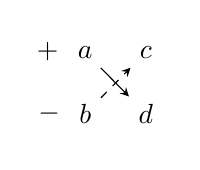
\begin{tikzpicture}[>=stealth]
            \matrix [%
                matrix of math nodes,
                column sep=1em,
                row sep=1em
            ] (s2) {%
                a & c \\
                b & d \\
            };

            \path
            (s2-1-1)    edge[->]        (s2-2-2)
            (s2-2-1)    edge[->,dashed] (s2-1-2);

            \node[anchor=east] at (s2-1-1.west) {\(+\)};
            \node[anchor=east] at (s2-2-1.west) {\(-\)};
        \end{tikzpicture}
    \end{figure*}
\end{example}

\begin{example}
    设 \(A\) 是一个 \(3\)~级阵.
    根据定义与上个例的结果,
    \begin{align*}
             & \det {(A)}
        \displaybreak[0]
        \\
        = {} &
        \hphantom{{} + {}}
        (-1)^{1+1} [A]_{1,1} \det {(A(1|1))}
        + (-1)^{2+1} [A]_{2,1} \det {(A(2|1))}
        \displaybreak[0]
        \\
             &
        + (-1)^{3+1} [A]_{3,1} \det {(A(3|1))}
        \displaybreak[0]
        \\
        = {} &
        \hphantom{{} + {}}
        [A]_{1,1}
        \det {\begin{bmatrix}
                      [A]_{2,2} & [A]_{2,3} \\
                      [A]_{3,2} & [A]_{3,3} \\
                  \end{bmatrix}}
        - [A]_{2,1}
        \det {\begin{bmatrix}
                      [A]_{1,2} & [A]_{1,3} \\
                      [A]_{3,2} & [A]_{3,3} \\
                  \end{bmatrix}}
        \displaybreak[0]
        \\
             &
        + [A]_{3,1}
        \det {\begin{bmatrix}
                      [A]_{1,2} & [A]_{1,3} \\
                      [A]_{2,2} & [A]_{2,3} \\
                  \end{bmatrix}}
        \displaybreak[0]
        \\
        = {} &
        \hphantom{{} + {}}
        [A]_{1,1}
        ([A]_{2,2} [A]_{3,3} - [A]_{3,2} [A]_{2,3})
        - [A]_{2,1}
        ([A]_{1,2} [A]_{3,3} - [A]_{3,2} [A]_{1,3})
        \displaybreak[0]
        \\
             &
        + [A]_{3,1}
        ([A]_{1,2} [A]_{2,3} - [A]_{2,2} [A]_{1,3})
        \displaybreak[0]
        \\
        = {} &
        \hphantom{{} + {}}
        [A]_{1,1} [A]_{2,2} [A]_{3,3}
        - [A]_{1,1} [A]_{3,2} [A]_{2,3}
        \displaybreak[0]
        \\
             &
        - [A]_{2,1} [A]_{1,2} [A]_{3,3}
        + [A]_{2,1} [A]_{3,2} [A]_{1,3}
        \displaybreak[0]
        \\
             &
        + [A]_{3,1} [A]_{1,2} [A]_{2,3}
        - [A]_{3,1} [A]_{2,2} [A]_{1,3}
        \displaybreak[0]
        \\
        = {} &
        \hphantom{{} + {}}
        [A]_{1,1} [A]_{2,2} [A]_{3,3}
        + [A]_{2,1} [A]_{3,2} [A]_{1,3}
        + [A]_{3,1} [A]_{1,2} [A]_{2,3}
        \displaybreak[0]
        \\
             &
        - [A]_{1,1} [A]_{3,2} [A]_{2,3}
        - [A]_{2,1} [A]_{1,2} [A]_{3,3}
        - [A]_{3,1} [A]_{2,2} [A]_{1,3}.
    \end{align*}
    法国数学人 Pierre Frédéric Sarrus
    \pinjino{salü}
    给了我们一个记 \(3\)~级阵的行列式的好方法.
    我们在阵的下面重写此阵.
    由左上至右下的对角线 (实线) 上的数的积的和%
    减由左下至右上的对角线 (虚线) 上的数的积的和%
    即为此阵的行列式.
    % https://tex.stackexchange.com/questions/32978/typesetting-a-matrix-with-crossing-arrows-on-it/#32981
    \begin{figure*}[h!]
        \centering
        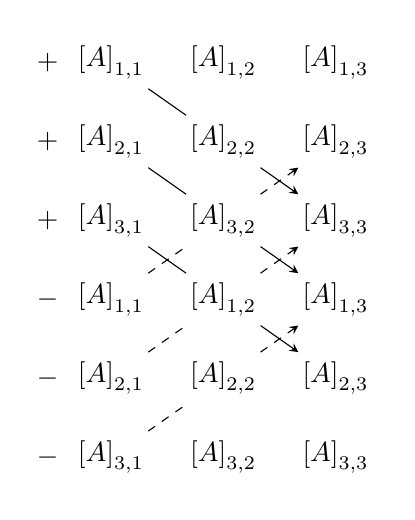
\begin{tikzpicture}[>=stealth]
            \matrix [%
            matrix of math nodes,
            column sep=1em,
            row sep=1em
            ] (s3) {%
            {[}A{]}_{1,1} & {[}A{]}_{1,2} & {[}A{]}_{1,3} \\
            {[}A{]}_{2,1} & {[}A{]}_{2,2} & {[}A{]}_{2,3} \\
            {[}A{]}_{3,1} & {[}A{]}_{3,2} & {[}A{]}_{3,3} \\
            {[}A{]}_{1,1} & {[}A{]}_{1,2} & {[}A{]}_{1,3} \\
            {[}A{]}_{2,1} & {[}A{]}_{2,2} & {[}A{]}_{2,3} \\
            {[}A{]}_{3,1} & {[}A{]}_{3,2} & {[}A{]}_{3,3} \\
            };

            \path
            (s3-1-1)    edge            (s3-2-2)
            (s3-2-2)    edge[->]        (s3-3-3)
            (s3-2-1)    edge            (s3-3-2)
            (s3-3-2)    edge[->]        (s3-4-3)
            (s3-3-1)    edge            (s3-4-2)
            (s3-4-2)    edge[->]        (s3-5-3)
            (s3-4-1)    edge[dashed]    (s3-3-2)
            (s3-3-2)    edge[->,dashed] (s3-2-3)
            (s3-5-1)    edge[dashed]    (s3-4-2)
            (s3-4-2)    edge[->,dashed] (s3-3-3)
            (s3-6-1)    edge[dashed]    (s3-5-2)
            (s3-5-2)    edge[->,dashed] (s3-4-3);

            \foreach \r in {1,2,3}
                {\node[anchor=east] at (s3-\r-1.west) {\(+\)};}
            \foreach \r in {4,5,6}
                {\node[anchor=east] at (s3-\r-1.west) {\(-\)};}
        \end{tikzpicture}
    \end{figure*}
\end{example}

不过, 注意,
前面的对角线法则无法被推广到
\(n\)~级阵 (\(n \geq 4\)) 的行列式.

\begin{example}
    设 \(A\) 是一个 \(4\)~级阵.
    根据定义,
    \begin{align*}
        %  &
        \det {(A)}
        % \\
        = {} &
        \hphantom{{} + {}}
        (-1)^{1+1} [A]_{1,1} \det {(A(1|1))}
        + (-1)^{2+1} [A]_{2,1} \det {(A(2|1))}
        \\
             &
        + (-1)^{3+1} [A]_{3,1} \det {(A(3|1))}
        + (-1)^{4+1} [A]_{4,1} \det {(A(4|1))}.
    \end{align*}
    利用跟上个例类似的方法, 并利用上个例的结果,
    可知, \(\det {(A)}\) 等于
    \begin{align*}
         & \hphantom{{} + {}}
        [A]_{1,1} [A]_{2,2} [A]_{3,3} [A]_{4,4}
        + [A]_{1,1} [A]_{3,2} [A]_{4,3} [A]_{2,4}
        + [A]_{1,1} [A]_{4,2} [A]_{2,3} [A]_{3,4}
        \\
         &
        - [A]_{1,1} [A]_{2,2} [A]_{4,3} [A]_{3,4}
        - [A]_{1,1} [A]_{3,2} [A]_{2,3} [A]_{4,4}
        - [A]_{1,1} [A]_{4,2} [A]_{3,3} [A]_{2,4}
        \\
         &
        - [A]_{2,1} [A]_{1,2} [A]_{3,3} [A]_{4,4}
        - [A]_{2,1} [A]_{3,2} [A]_{4,3} [A]_{1,4}
        - [A]_{2,1} [A]_{4,2} [A]_{1,3} [A]_{3,4}
        \\
         &
        + [A]_{2,1} [A]_{1,2} [A]_{4,3} [A]_{3,4}
        + [A]_{2,1} [A]_{3,2} [A]_{1,3} [A]_{4,4}
        + [A]_{2,1} [A]_{4,2} [A]_{3,3} [A]_{1,4}
        \\
         &
        + [A]_{3,1} [A]_{1,2} [A]_{2,3} [A]_{4,4}
        + [A]_{3,1} [A]_{2,2} [A]_{4,3} [A]_{1,4}
        + [A]_{3,1} [A]_{4,2} [A]_{1,3} [A]_{2,4}
        \\
         &
        - [A]_{3,1} [A]_{1,2} [A]_{4,3} [A]_{2,4}
        - [A]_{3,1} [A]_{2,2} [A]_{1,3} [A]_{4,4}
        - [A]_{3,1} [A]_{4,2} [A]_{2,3} [A]_{1,4}
        \\
         &
        - [A]_{4,1} [A]_{1,2} [A]_{2,3} [A]_{3,4}
        - [A]_{4,1} [A]_{2,2} [A]_{3,3} [A]_{1,4}
        - [A]_{4,1} [A]_{3,2} [A]_{1,3} [A]_{2,4}
        \\
         &
        + [A]_{4,1} [A]_{1,2} [A]_{3,3} [A]_{2,4}
        + [A]_{4,1} [A]_{2,2} [A]_{1,3} [A]_{3,4}
        \underline{{}
        + [A]_{4,1} [A]_{3,2} [A]_{2,3} [A]_{1,4}}.
    \end{align*}
    根据对角线法则,
    我们似乎应减由左下至右上的对角线上的数的积.
    可是, 由上式,
    \([A]_{4,1} [A]_{3,2} [A]_{2,3} [A]_{1,4}\)
    前的符号是 \(+\),
    而不是 \(-\).
    \begin{figure*}[h!]
        \centering
        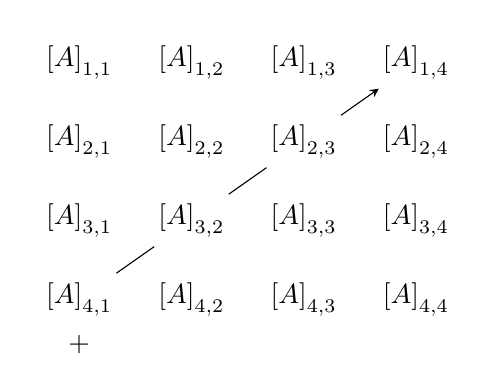
\begin{tikzpicture}[>=stealth]
            \matrix [%
            matrix of math nodes,
            column sep=1em,
            row sep=1em
            ] (s4) {%
            {[}A{]}_{1,1} & {[}A{]}_{1,2} &
            {[}A{]}_{1,3} & {[}A{]}_{1,4} \\
            {[}A{]}_{2,1} & {[}A{]}_{2,2} &
            {[}A{]}_{2,3} & {[}A{]}_{2,4} \\
            {[}A{]}_{3,1} & {[}A{]}_{3,2} &
            {[}A{]}_{3,3} & {[}A{]}_{3,4} \\
            {[}A{]}_{4,1} & {[}A{]}_{4,2} &
            {[}A{]}_{4,3} & {[}A{]}_{4,4} \\
            };

            \path
            % (s4-4-1)    edge[dashed]    (s4-3-2)
            % (s4-3-2)    edge[dashed]    (s4-2-3)
            % (s4-2-3)    edge[->,dashed] (s4-1-4);
            (s4-4-1)    edge[]    (s4-3-2)
            (s4-3-2)    edge[]    (s4-2-3)
            (s4-2-3)    edge[->]  (s4-1-4);

            \node[anchor=north] at (s4-4-1.south)
            % {It is \(+\).};
            {\(+\)};
        \end{tikzpicture}
    \end{figure*}

    我不要求您记如此具体的公式,
    因为 \(n\)~级阵 (\(n \geq 4\)) 的行列式的具体的公式%
    不如 \(1\)~级阵, \(2\)~级阵, \(3\)~级阵%
    的行列式的具体的公式实用.
\end{example}

\section{按一列展开行列式}

前面, 我们学习了行列式:

\DefinitionDeterminants*

不难看出,
\([A]_{1,1}\), \([A]_{2,1}\), \(\dots\), \([A]_{n,1}\)
全为 \(A\)~的列~\(1\) 的元,
故我们说,
定义按列~\(1\) 展开行列式.
自然地, 我们会想,
我们能否按别的列展开行列式.
此事的回答是 ``是''.
具体地, 我们有

% restatable that one has manually to repeat
% in at least one other file:
% determinanto - ecoj de determinantoj.tex
% determinanto - matrica multipliko.tex
\begin{restatable}{theorem}{TheoremExpansionAboutAnyColumn}
    设 \(A\) 是 \(n\)~级阵 (\(n \geq 1\)).
    设 \(j\) 为整数, 且 \(1 \leq j \leq n\).
    则
    \begin{align*}
        \det {(A)} = \sum_{i = 1}^{n}
        {(-1)^{i+j} [A]_{i,j} \det {(A(i|j))}}.
    \end{align*}
\end{restatable}

% 或许, 我应解释,
% 当 \(A\) 是 \(1\)~级阵时,
% \(\det {(A(1|1))}\) 是什么.
% 显然, 去除 \(A\) 的唯一的一行与唯一的一列后,
% 就不剩下元了.
% 我给出的阵的定义显然未包含此情形.
% 我给出的行列式的定义也未包含此情形.
% 我们作一个约定:
% \(1\)~级阵 \(A\) 的子阵 \(A(1|1)\) 是 \emph{``\(0\)~级阵''},
% 且 ``\(0\)~级阵'' 的行列式是 \(1\).
% 这么看来, \((-1)^{1+1} [A]_{1,1} \det {(A(1|1))}\)
% 就是 \(1 \cdot [A]_{1,1} \cdot 1\),
% 即 \([A]_{1,1}\),
% 跟行列式的定义一样.

或许, 我应解释,
当 \(A\) 是 \(1\)~级阵时,
\(\det {(A(1|1))}\) 是什么.
显然, 去除 \(A\) 的一行与一列后,
就不剩下元了.
``\(A(1|1)\)'' 也不再是一个阵.
不过, 我们作约定:
\(1\)~级阵 \(A\) 的子阵 \(A(1|1)\) 是 \emph{``\(0\)~级阵''},
且 ``\(0\)~级阵'' 的行列式是 \(1\).
这么看来, \((-1)^{1+1} [A]_{1,1} \det {(A(1|1))}\)
就是 \(1 \cdot [A]_{1,1} \cdot 1\),
即 \([A]_{1,1}\).
% 跟行列式的定义一样.
% (回想, 类似地, 一个 (非零的) 数的
% \(0\)~次方被约定为 \(1\).)

我们无妨先用 \(2\)~级阵验证此命题.
设 \(A\) 是 \(2\)~级阵 (也就是, 取 \(n = 2\)).
\(j = 1\) 时, 这就是定义;
\(j = 2\) 时,
\begin{align*}
    \det {(A)}
    = {} &
    [A]_{1,1} [A]_{2,2} - [A]_{2,1} [A]_{1,2}
    \\
    = {} &
    {-} [A]_{1,2} [A]_{2,1} + [A]_{2,2} [A]_{1,1}
    \\
    = {} &
    (-1)^{1+2} [A]_{1,2} \det {(A(1|2))}
    + (-1)^{2+2} [A]_{2,2} \det {(A(2|2))}.
\end{align*}
所以, \(n = 2\) 时, 命题是对的.

\begin{proof}
    我们会用数学归纳法证明此事.
    具体地, 设 \(P(n)\) 为命题
    \begin{quotation}
        对任何 \(n\)~级阵 \(A\),
        对任何不超过 \(n\) 的正整数 \(j\),
        \begin{align*}
            \det {(A)} = \sum_{i = 1}^{n}
            {(-1)^{i+j} [A]_{i,j} \det {(A(i|j))}}.
        \end{align*}
    \end{quotation}
    则, 我们的目标是,
    对任何正整数 \(n\), \(P(n)\) 是对的.

    用数学归纳法不应是一个意外:
    我给出的行列式的定义就是%
    先定义小级阵的行列式,
    再用小级阵的行列式定义大级阵的行列式.

    设 \(n = 1\).
    \(j = 1\) 时, 显然.
    故 \(P(1)\) 是对的.

    设 \(n = 2\).
    \(j = 1\) 时, 也显然 (定义).
    \(j = 2\) 时, 我们已验证它.
    故 \(P(2)\) 是对的.

    现在, 我们假定 \(P(m-1)\) 是对的.
    我们要证 \(P(m)\) 也是对的.
    任取一个 \(m\)~级阵 \(A\).
    若 \(j = 1\), 这是定义.
    现设 \(j \neq 1\).
    为方便, 对二个整数 \(i\), \(j\), 我们定义
    \begin{align*}
        \rho(i, j)
        = \begin{cases}
              0, & i < j;    \\
              1, & i \geq j.
          \end{cases}
    \end{align*}
    于是
    \begingroup
    \reqnomode
    \begin{align*}
             & \det {(A)}                  \\
        = {} &
        \sum_{i = 1}^{m} {
        (-1)^{i+1} [A]_{i,1} \det {(A(i|1))}
        }
        \tag*{(1)}
        \\
        = {} &
        \sum_{i = 1}^{m} {
        (-1)^{i+1} [A]_{i,1}
        \sum_{\substack{1 \leq \ell \leq m \\ \ell \neq i}} {
        (-1)^{(\ell - \rho(\ell, i)) + (j - 1)}
            [A]_{\ell,j} \det {(A({i,\ell}|{1,j}))}
        }
        }
        \tag*{(2)}
        \\
        = {} &
        \sum_{i = 1}^{m} {
        \sum_{\substack{1 \leq \ell \leq m \\ \ell \neq i}} {
        (-1)^{(\ell - \rho(\ell, i)) + (j - 1)}
        (-1)^{i+1}
            [A]_{i,1} [A]_{\ell,j} \det {(A({i,\ell}|{1,j}))}
        }
        }
        \tag*{(3)}
        \\
        = {} &
        \sum_{\ell = 1}^{m} {
        \sum_{\substack{1 \leq i \leq m    \\ i \neq \ell}} {
        (-1)^{(\ell - \rho(\ell, i)) + (j - 1)}
        (-1)^{i+1}
            [A]_{i,1} [A]_{\ell,j} \det {(A({i,\ell}|{1,j}))}
        }
        }
        \tag*{(4)}
        \\
        = {} &
        \sum_{\ell = 1}^{m} {
        \sum_{\substack{1 \leq i \leq m    \\ i \neq \ell}} {
        (-1)^{\ell} (-1)^{\rho(\ell, i)} (-1)^{i} (-1)^{j}
            [A]_{i,1} [A]_{\ell,j} \det {(A({i,\ell}|{1,j}))}
        }
        }
        \tag*{(5)}
        \\
        = {} &
        \sum_{\ell = 1}^{m} {
        \sum_{\substack{1 \leq i \leq m    \\ i \neq \ell}} {
        (-1)^{\ell + j} (-1)^{i - \rho(i, \ell) + 1}
            [A]_{i,1} [A]_{\ell,j} \det {(A({i,\ell}|{1,j}))}
        }
        }
        \tag*{(6)}
        \\
        = {} &
        \sum_{\ell = 1}^{m} {(-1)^{\ell + j} [A]_{\ell,j}
        \sum_{\substack{1 \leq i \leq m    \\ i \neq \ell}} {
        (-1)^{i - \rho(i, \ell) + 1}
            [A]_{i,1} \det {(A({i,\ell}|{1,j}))}
        }
        }
        \tag*{(7)}
        \\
        = {} &
        \sum_{\ell = 1}^{m} {(-1)^{\ell + j} [A]_{\ell,j}
        \det {(A(\ell|j))}
        }.
        \tag*{(8)}
    \end{align*}
    \endgroup
    所以, \(P(m)\) 是对的.
    由数学归纳法, 待证命题成立.

    我想, 您看到了公式右侧的序号.
    这是方便我说话用的.
    我想, 适当地解释这几步是好的.

    (1) 是行列式的定义.

    (2) 利用了假定.
    我们假定可按任何列展开%
    任何 \(m - 1\)~级阵的行列式.
    \(A(i|1)\) 不就是 \(m - 1\)~级阵吗?
    那么, 我们就按 \(A(i|1)\) 的列~\(j - 1\) 展开.
    \(A(i|1)\) 的列~\(j - 1\) 正好对应
    \(A\) 的列~\(j\).
    最后, 注意, \(\ell \neq i\) 时,
    \(A\)~的 \((\ell, j)\)-元恰是
    \(A(i|1)\)~的 \((\ell - \rho(\ell, i), j - 1)\)-元.

    (3) 利用了分配律 (还有加法的结合律与交换律).

    (4) 利用了加法的结合律与交换律.
    (通俗地, 求和号的次序可换.)

    (5) 利用了 \(-1\)~的整数次方的性质.

    (6) 还是利用 \(-1\)~的整数次方的性质.
    注意, \(i \neq \ell\) 时,
    \(\rho(i, \ell) + \rho(\ell, i) = 1\).

    (7) 再用了一次分配律 (还有加法的结合律与交换律).
    不过, 跟 (3) 对比, 这次是反过来用.

    (8) 用到了行列式的定义.
    注意, \(i \neq \ell\) 时,
    \(A\)~的 \((i, 1)\)-元恰是
    \(A(\ell|j)\)~的 \((i - \rho(i, \ell), 1)\)-元
    (其中, \(j \neq 1\)).
\end{proof}

\KunAsteriskoEnEnhavtabelo
\section{按多列展开行列式}
\SenAsteriskoEnEnhavtabelo

\maldevigalegajxo

前面, 我们知道, 我们可按 (任何) 一列展开行列式:

\TheoremExpansionAboutAnyColumn*

自然地, 我们会想, 我们能否按多列展开行列式.
此事的回答是 ``是''.
具体地, 我们有

\begin{theorem}
    设 \(A\) 是 \(n\)~级阵 (\(n \geq 1\)).
    设 \(k\) 是不超过 \(n\) 的正整数.
    设 \(j_1\), \(j_2\), \(\dots\), \(j_k\) 是%
    不超过 \(n\) 的正整数,
    且 \(j_1 < j_2 < \dots < j_k\).
    则
    \begin{align*}
         &
        \det {(A)}
        = \sum_{1 \leq i_1 < i_2 < \dots < i_k \leq n}
        {\det {\left(
                A\binom{i_1, i_2, \dots, i_k}
                {j_1, j_2, \dots, j_k}
                \right)}}
        \\
         &
        \qquad \qquad \qquad
        \cdot (-1)^{i_1 + i_2 + \dots + i_k
            + j_1 + j_2 + \dots + j_k}
        \det {(A({i_1,i_2,\dots,i_k}|{j_1,j_2,\dots,j_k}))}.
    \end{align*}
\end{theorem}

若 \(k = 1\), 则
\(\displaystyle
A\binom{i_1}{j_1} = [[A]_{i_1,j_1}]\)
是一个 \(1\)~级阵.
回想, \(1\)~级阵 \([a]\) 的行列式就是 \(a\).
所以, 若 \(k = 1\), 则此定理就是%
按一列展开行列式.

论证此事前, 我想用一个例助您理解, 此定理在说什么.

\begin{example}
    设
    \begin{align*}
        A =
        \begin{bmatrix}
            1 & 5 & 8  & 16 \\
            2 & 6 & 10 & 15 \\
            3 & 7 & 11 & 13 \\
            4 & 9 & 12 & 14 \\
        \end{bmatrix}.
    \end{align*}

    一方面,
    根据定义,
    \begin{align*}
        %  &
        \det {(A)}
        %  \\
        = {} &
        \hphantom{{} + {}}
        (-1)^{1+1} [A]_{1,1} \det {(A(1|1))}
        + (-1)^{2+1} [A]_{2,1} \det {(A(2|1))}
        \\
             &
        + (-1)^{3+1} [A]_{3,1} \det {(A(3|1))}
        + (-1)^{4+1} [A]_{4,1} \det {(A(4|1))}.
    \end{align*}
    则
    \begin{align*}
         & \det {(A(1|1))}
        = \det {\begin{bmatrix}
                        6 & 10 & 15 \\
                        7 & 11 & 13 \\
                        9 & 12 & 14 \\
                    \end{bmatrix}}
        = -47;             \\
         & \det {(A(2|1))}
        = \det {\begin{bmatrix}
                        5 & 8  & 16 \\
                        7 & 11 & 13 \\
                        9 & 12 & 14 \\
                    \end{bmatrix}}
        = -98;             \\
         & \det {(A(3|1))}
        = \det {\begin{bmatrix}
                        5 & 8  & 16 \\
                        6 & 10 & 15 \\
                        9 & 12 & 14 \\
                    \end{bmatrix}}
        = -80;             \\
         & \det {(A(4|1))}
        = \det {\begin{bmatrix}
                        5 & 8  & 16 \\
                        6 & 10 & 15 \\
                        7 & 11 & 13 \\
                    \end{bmatrix}}
        = -23.
    \end{align*}
    所以
    \begin{align*}
        \det {(A)}
        = 1 \cdot (-47) - 2 \cdot (-98)
        + 3 \cdot (-80) - 4 \cdot (-23)
        = 1.
    \end{align*}

    另一方面,
    我们试按列~\(1\), \(2\) 展开.
    取 \(j_1\), \(j_2\) 为 \(1\), \(2\).
    不难写出, 适合条件
    ``\(1 \leq i_1 < i_2 \leq 4\)''
    的 \((i_1, i_2)\) 有 \(6\)~个:
    \((1, 2)\),
    \((1, 3)\), \((2, 3)\),
    \((1, 4)\), \((2, 4)\), \((3, 4)\).
    则
    \begin{align*}
         & A\binom{1,2}{1,2}
        = \begin{bmatrix}1&5\\2&6\\ \end{bmatrix},
        \quad
        (-1)^{1+2+1+2} = +1,
        \quad
        A(1,2|1,2)
        = \begin{bmatrix}11&13\\12&14\\ \end{bmatrix};
        \\
         & A\binom{1,3}{1,2}
        = \begin{bmatrix}1&5\\3&7\\ \end{bmatrix},
        \quad
        (-1)^{1+3+1+2} = -1,
        \quad
        A(1,3|1,2)
        = \begin{bmatrix}10&15\\12&14\\ \end{bmatrix};
        \\
         & A\binom{2,3}{1,2}
        = \begin{bmatrix}2&6\\3&7\\ \end{bmatrix},
        \quad
        (-1)^{2+3+1+2} = +1,
        \quad
        A(2,3|1,2)
        = \begin{bmatrix}8&16\\12&14\\ \end{bmatrix};
        \\
         & A\binom{1,4}{1,2}
        = \begin{bmatrix}1&5\\4&9\\ \end{bmatrix},
        \quad
        (-1)^{1+4+1+2} = +1,
        \quad
        A(1,4|1,2)
        = \begin{bmatrix}10&15\\11&13\\ \end{bmatrix};
        \\
         & A\binom{2,4}{1,2}
        = \begin{bmatrix}2&6\\4&9\\ \end{bmatrix},
        \quad
        (-1)^{2+4+1+2} = -1,
        \quad
        A(2,4|1,2)
        = \begin{bmatrix}8&16\\11&13\\ \end{bmatrix};
        \\
         & A\binom{3,4}{1,2}
        = \begin{bmatrix}3&7\\4&9\\ \end{bmatrix},
        \quad
        (-1)^{3+4+1+2} = +1,
        \quad
        A(3,4|1,2)
        = \begin{bmatrix}8&16\\10&15\\ \end{bmatrix}.
    \end{align*}
    定理说,
    \begin{align*}
        \det {(A)}
        = {} & \hphantom{{} + {}}
        \det {\left( A\binom{1,2}{1,2} \right)}\,
        (-1)^{1+2+1+2} \det {(A(1,2|1,2))}
        \\
             & + \det {\left( A\binom{1,3}{1,2} \right)}\,
        (-1)^{1+3+1+2} \det {(A(1,3|1,2))}
        \\
             & + \det {\left( A\binom{2,3}{1,2} \right)}\,
        (-1)^{2+3+1+2} \det {(A(2,3|1,2))}
        \\
             & + \det {\left( A\binom{1,4}{1,2} \right)}\,
        (-1)^{1+4+1+2} \det {(A(1,4|1,2))}
        \\
             & + \det {\left( A\binom{2,4}{1,2} \right)}\,
        (-1)^{2+4+1+2} \det {(A(2,4|1,2))}
        \\
             & + \det {\left( A\binom{3,4}{1,2} \right)}\,
        (-1)^{3+4+1+2} \det {(A(3,4|1,2))}
        \\
        = {} & \hphantom{{} + {}}
        (-4) \cdot (-2) - (-8) \cdot (-40)
        \\
             & + (-4) \cdot (-80) + (-11) \cdot (-35)
        \\
             & - (-6) \cdot (-72) + (-1) \cdot (-40)
        \\
        = {} & 8 - 320 + 320 + 385 - 432 + 40
        \\
        = {} & 1.
    \end{align*}
\end{example}

\begin{proof}
    我们用数学归纳法证明此事.
    具体地, 设 \(P(k)\) 为命题
    \begin{quotation}
        对任何 \(n\)~级阵 \(A\)
        (其中, \(n \geq k\)),
        对任何不超过 \(n\) 的 \(k\) 个正整数
        \(j_1\), \(j_2\), \(\dots\), \(j_k\)
        (其中, \(j_1 < j_2 < \dots < j_k\)),
        \begin{align*}
             &
            \det {(A)}
            = \sum_{1 \leq i_1 < i_2 < \dots < i_k \leq n}
            {\det {\left(
                    A\binom{i_1, i_2, \dots, i_k}%
                    {j_1, j_2, \dots, j_k}
                    \right)}}
            \\
             &
            \qquad \qquad \qquad
            \cdot (-1)^{i_1 + i_2 + \dots + i_k
                + j_1 + j_2 + \dots + j_k}
            \det {(A({i_1,i_2,\dots,i_k}|{j_1,j_2,\dots,j_k}))}.
        \end{align*}
    \end{quotation}
    则, 我们的目标是,
    对任何正整数 \(k\), \(P(k)\) 是对的.

    \(k = 1\) 时, 这就是按一列展开行列式.

    现在, 我们假定 \(P(k - 1)\) 是对的.
    我们要证 \(P(k)\) 也是对的.
    任取一个 \(n\)~级阵~\(A\) (\(n \geq k\)).
    任取不超过 \(n\) 的正整数
    \(j_1\), \(j_2\), \(\dots\), \(j_k\),
    且 \(j_1 < j_2 < \dots < j_k\).
    按列~\(j_1\) 展开行列式,
    知
    \begin{align*}
        \det {(A)} = \sum_{d_1 = 1}^{n}
        {[A]_{d_1,j_1}
        (-1)^{d_1 + j_1}
        \det {(A(d_1|j_1))}}.
    \end{align*}

    注意,
    \(A\)~的列~\(j_2\), \(j_3\), \(\dots\), \(j_k\)
    跟 \(A(d_1|j_1)\) 的列~\(j_2 - 1\),
    \(j_3 - 1\), \(\dots\), \(j_k - 1\)
    对应,
    且 \(A\)~的行~\(i\) (\(i \neq d_1\))
    跟 \(A(d_1|j_1)\)~的行~\(i - \rho(i, d_1)\) 对应.
    利用假定,
    我们按列~\(j_2 - 1\), \(j_3 - 1\), \(\dots\), \(j_k - 1\)
    展开每个 \(\det {(A(d_1|j_1))}\),
    有
    \begin{align*}
         &
        \det {(A(d_1|j_1))}
        = \sum_{\substack{
        1 \leq d_2 < \dots < d_k \leq n \\
                d_1 \neq d_2,\dots,d_k
            }}
        {\det {\left(
                A\binom{d_2, \dots, d_k}{j_2, \dots, j_k}
                \right)}}
        \\
         &
        \qquad \qquad \qquad \qquad \qquad
        \cdot (-1)^{d_2 - \rho(d_2, d_1) + \dots
            + d_k - \rho(d_k, d_1)
            + j_2 + \dots + j_k - (k - 1)}
        \\
         &
        \qquad \qquad \qquad \qquad \qquad
        \cdot \det
        {(A({d_1,d_2,\dots,d_k}|{j_1,j_2,\dots,j_k}))}.
    \end{align*}
    利用分配律 (还有加法的结合律与交换律), 有
    \begin{align*}
         &
        \det {(A)}
        = \sum_{\substack{
        1 \leq d_1 \leq n               \\
        1 \leq d_2 < \dots < d_k \leq n \\
                d_1 \neq d_2,\dots,d_k
            }}
        {[A]_{d_1,j_1}
            (-1)^{d_1 + j_1}
            \det {\left(
                A\binom{d_2, \dots, d_k}{j_2, \dots, j_k}
                \right)}}
        \\
         &
        \qquad \qquad \qquad \qquad
        \cdot (-1)^{d_2 - \rho(d_2, d_1) + \dots
            + d_k - \rho(d_k, d_1)
            + j_2 + \dots + j_k - (k - 1)}
        \\
         &
        \qquad \qquad \qquad \qquad
        \cdot \det {(A({d_1,d_2,\dots,d_k}|{j_1,j_2,\dots,j_k}))}.
    \end{align*}
    注意,
    \begin{align*}
             &
        d_1 + j_1 + d_2 - \rho(d_2, d_1) + \dots
        + d_k - \rho(d_k, d_1)
        + j_2 + \dots + j_k - (k - 1)
        \\
        = {} &
        \hphantom{{} + {}}
        (d_1 + \dots + d_k) + (j_1 + \dots + d_k)
        \\
             &
        + (\rho(d_1, d_2) - 1) + \dots + (\rho(d_1, d_k) - 1)
        - (k - 1)
        \\
        = {} &
        (d_1 + \dots + d_k) + (j_1 + \dots + j_k)
        + (\rho(d_1, d_2) + \dots + \rho(d_1, d_k))
        - 2(k-1).
    \end{align*}
    故
    \begin{align*}
         &
        \det {(A)}
        = \sum_{\substack{
        1 \leq d_1 \leq n               \\
        1 \leq d_2 < \dots < d_k \leq n \\
                d_1 \neq d_2,\dots,d_k
            }}
        {(-1)^{\rho(d_1, d_2) + \dots + \rho(d_1, d_k)}
                [A]_{d_1,j_1}
            \det {\left(
                A\binom{d_2, \dots, d_k}{j_2, \dots, j_k}
                \right)}}
        \\
         &
        \qquad \qquad \qquad
        \cdot (-1)^{d_1 + \dots + d_k + j_1 + \dots + j_k}
        \det {(A({d_1,d_2,\dots,d_k}|{j_1,j_2,\dots,j_k}))}.
    \end{align*}

    % \begingroup

    % \makeatletter
    % % https://tex.stackexchange.com/questions/198771/align-in-substack
    % \providecommand*{\subalign}[1]{%
    %     \vcenter{%
    %         \Let@ \restore@math@cr \default@tag
    %         \baselineskip\fontdimen10 \scriptfont\tw@
    %         \advance\baselineskip\fontdimen12 \scriptfont\tw@
    %         \lineskip\thr@@\fontdimen8 \scriptfont\thr@@
    %         \lineskiplimit\lineskip
    %         \ialign{\hfil\(\m@th\scriptstyle##\)&%
    %             \(\m@th\scriptstyle{}##\)\hfil\crcr
    %             #1\crcr
    %         }%
    %     }%
    % }
    % \makeatother

    注意,
    \begin{align*}
        \sum_{\substack{
        1 \leq d_1 \leq n               \\
        1 \leq d_2 < \dots < d_k \leq n \\
                d_1 \neq d_2,\dots,d_k
            }} {f(d_1, \dots, d_k)}
        =
        \sum_{1 \leq i_1 < i_2 < \dots < i_k \leq n}
        { \sum_{\substack{
        1 \leq s \leq k                 \\
        d_1 = i_s                       \\
                    d_r = i_{r - \rho(s, r)}\,(2 \leq r \leq k)
                }}
            {f(d_1, \dots, d_k)}}.
    \end{align*}
    我解释此式.
    要从 \(1\) 至 \(n\) 这 \(n\)~个整数中选出 \(k\)~个数
    \(d_1\), \(d_2\), \(\dots\), \(d_k\),
    适合条件 \(d_2 < \dots < d_k\),
    且 \(d_1\) 不跟 \(d_2\), \(\dots\), \(d_k\) 的任何一个相等,
    我们可以先从
    \(1\), \(2\), \(\dots\), \(n\) 里从小到大地%
    挑 \(k\)~个数 \(i_1\), \(i_2\), \(\dots\), \(i_k\),
    然后从 \(i_1\), \(i_2\), \(\dots\), \(i_k\)
    选第~\(s\) 小的数 \(i_s\) 为 \(d_1\),
    且分别取
    \(d_2\), \(d_3\), \(\dots\), \(d_k\)
    为
    \(i_1\), \(\dots\), \(i_{s-1}\),
    \(i_{s+1}\), \(\dots\), \(i_{k}\).
    (若 \(s = 1\), 则不出现 \(i_1\);
    若 \(s = k\), 则不出现 \(i_k\).
    下同.)
    更具体地, 我们使 \(d_1\) 为 \(i_s\),
    再使 \(d_r\) (\(r \geq 2\)) 为 \(i_{\ell (r)}\),
    其中, \(2 \leq r \leq s\) 时 \(\ell (r) = r-1\),
    而 \(r > s\) 时 \(\ell (r) = r\).
    利用 \(\rho\)-记号, 就是 \(d_1 = i_s\),
    且 \(d_r = i_{r - \rho(s, r)}\) (\(2 \leq r \leq k\)).

    % \endgroup

    当 \(d_1 = i_s\),
    且 \(d_r = i_{r - \rho(s, r)}\)
    (\(2 \leq r \leq k\)) 时,
    \begin{align*}
         &
        d_1 = i_s,
        \\
         &
        \rho(d_1, d_2) + \dots + \rho(d_1, d_k)
        = s - 1 = (s + 1) - 2,
        \\
         &
        [A]_{d_1,j_1} = [A]_{i_s,j_1},
        \\
         &
        A\binom{d_2, \dots, d_k}{j_2, \dots, j_k}
        =
        A\binom{i_1, \dots, i_{s-1}, i_{s+1}, \dots, i_k}
        {j_2, \dots, j_k},
        \\
         &
        d_1 + \dots + d_k = i_1 + \dots + i_k,
        \\
         &
        A({d_1,d_2,\dots,d_k}|{j_1,j_2,\dots,j_k})
        =
        A({i_1,i_2,\dots,i_k}|{j_1,j_2,\dots,j_k}).
    \end{align*}
    故
    \begin{align*}
             &
        \det {(A)}
        \\
        = {} &
        \sum_{1 \leq i_1 < i_2 < \dots < i_k \leq n}
        {\sum_{1 \leq s \leq k}
            {(-1)^{s+1} [A]_{i_s,j_1}
                \det {\left(
                    A\binom{i_1, \dots, i_{s-1},
                        i_{s+1}, \dots, i_k}
                    {j_2, \dots, j_k}
                    \right)}}}
        \\
             &
        \qquad \qquad \qquad
        \cdot
        (-1)^{i_1 + \dots + i_k + j_1 + \dots + j_k}
        \det {(A({i_1,i_2,\dots,i_k}|{j_1,j_2,\dots,j_k}))}.
    \end{align*}
    注意, \(i_1 + \dots + i_k\) 与
    \(A({i_1,i_2,\dots,i_k}|{j_1,j_2,\dots,j_k})\)
    都跟 \(s\) 无关,
    故由分配律 (还有加法的结合律与交换律),
    \begin{align*}
             &
        \det {(A)}
        \\
        = {} &
        \sum_{1 \leq i_1 < i_2 < \dots < i_k \leq n}
        {\left(
            \sum_{1 \leq s \leq k}
            {(-1)^{s+1} [A]_{i_s,j_1}
                \det {\left(
                    A\binom{i_1, \dots, i_{s-1},
                        i_{s+1}, \dots, i_k}
                    {j_2, \dots, j_k}
                    \right)}}
            \right)}
        \\
             &
        \qquad \qquad \qquad
        \cdot
        (-1)^{i_1 + \dots + i_k + j_1 + \dots + j_k}
        \det {(A({i_1,i_2,\dots,i_k}|{j_1,j_2,\dots,j_k}))}.
    \end{align*}
    注意, \([A]_{i_s,j_1}\) 是
    \(\displaystyle
    A\binom{i_1, \dots, i_k}
    {j_1, \dots, j_k}\)~的
    \((s, 1)\)-元, 故
    \begin{align*}
             & \sum_{1 \leq s \leq k}
        {(-1)^{s+1} [A]_{i_s,j_1}
            \det {\left(
                A\binom{i_1, \dots, i_{s-1}, i_{s+1}, \dots, i_k}
                {j_2, \dots, j_k}
                \right)}}
        \\
        = {} & \det {\left(
            A\binom{i_1, \dots, i_k}
            {j_1, \dots, j_k}
            \right)}.
    \end{align*}
    综上, 我们有
    \begin{align*}
         &
        \det {(A)}
        = \sum_{1 \leq i_1 < i_2 < \dots < i_k \leq n}
        {\det {\left(
                A\binom{i_1, i_2, \dots, i_k}
                {j_1, j_2, \dots, j_k}
                \right)}}
        \\
         &
        \qquad \qquad \qquad
        \cdot (-1)^{i_1 + i_2 + \dots + i_k
            + j_1 + j_2 + \dots + j_k}
        \det {(A({i_1,i_2,\dots,i_k}|{j_1,j_2,\dots,j_k}))}.
    \end{align*}
    所以, \(P(k)\) 是对的.
    由数学归纳法, 待证命题成立.
\end{proof}

\KunAsteriskoEnEnhavtabelo
\section{完全展开行列式}
\SenAsteriskoEnEnhavtabelo

\maldevigalegajxo

前面, 我们研究了按一列展开行列式.
它变大级阵的行列式为一些小级阵的行列式.
本节, 我们考虑完全展开行列式.
它直接地用阵的元写出行列式的具体的公式.

其实, 我给出行列式的定义后,
我们立即算出了小级阵 (不超过 \(4\))
的行列式的具体的公式.
\(1\)~级阵的行列式非常简单, 且有 \(1\)~项;
\(2\)~级阵的行列式不难, 且有 \(2\)~项;
\(3\)~级阵的行列式较难, 且有 \(6\)~项;
\(4\)~级阵的行列式更复杂, 且有 \(24\)~项.
一般地, 我们有

% restatable that one has manually to repeat
% in at least one other file:
% determinanto - BC.tex
\begin{restatable}{theorem}{TheoremFullExpansion}
    设 \(A\) 是 \(n\)~级阵 (\(n \geq 1\)).
    设 \(j_1\), \(j_2\), \(\dots\), \(j_n\) 是%
    不超过 \(n\) 的正整数,
    且互不相同.
    则
    \begin{align*}
             & \det {(A)}
        \\
        = {} &
        \sum_{\substack{
        1 \leq i_1, i_2, \dots, i_n \leq n \\
                i_1, i_2, \dots, i_n\,\text{互不相同}
            }}
        {s(i_1, i_2, \dots, i_n)\,
            s(j_1, j_2, \dots, j_n)\,
            [A]_{i_1,j_1} [A]_{i_2,j_2} \dots [A]_{i_n,j_n}}.
    \end{align*}
    特别地, 取 \(j_1\), \(j_2\), \(\dots\), \(j_n\)
    为 \(1\), \(2\), \(\dots\), \(n\),
    并注意, \(s(1, 2, \dots, n) = 1\),
    得
    \begin{align*}
        \det {(A)}
        = {} &
        \sum_{\substack{
        1 \leq i_1, i_2, \dots, i_n \leq n \\
                i_1, i_2, \dots, i_n\,\text{互不相同}
            }}
        {s(i_1, i_2, \dots, i_n)\,
            [A]_{i_1,1} [A]_{i_2,2} \dots [A]_{i_n,n}}.
    \end{align*}
\end{restatable}

\begin{proof}
    我们按列~\(j_1\) 展开 \(\det {(A)}\),
    有
    \begin{align*}
        \det {(A)}
        = \sum_{1 \leq i_1 \leq n}
        {(-1)^{i_1 + j_1} [A]_{i_1,j_1} \det {(A(i_1|j_1))}}.
    \end{align*}

    注意, \(A\)~的列~\(j_2\) 对应
    \(A(i_1|j_1)\)~的列~\(j_2 - \rho(j_2, j_1)\),
    且 \(A\)~的行~\(i_2\) (\(i_2 \neq i_1\)) 对应
    \(A(i_1|j_1)\)~的行~\(i_2 - \rho(i_2, i_1)\).
    再注意,
    \begin{align*}
        i_2 - \rho(i_2, i_1) + j_2 - \rho(j_2, j_1)
        = i_2 + j_2 + \rho(i_1, i_2) + \rho(j_1, j_2) - 2,
    \end{align*}
    故
    \begin{align*}
             &
        \det {(A(i_1|j_1))}
        \\
        = {} &
        \sum_{\substack{
        1 \leq i_2 \leq n \\
            i_2 \neq i_1
        }}
        {(-1)^{i_2 + j_2 + \rho(i_1, i_2) + \rho(j_1, j_2)}
            [A]_{i_2,j_2} \det {(A({i_1,i_2}|{j_1,j_2}))}}.
    \end{align*}

    ……

    注意, \(A\)~的列~\(j_k\) 对应
    \(A({i_1,\dots,i_{k-1}}|{j_1,\dots,j_{k-1}})\)~的%
    列~\(j_k - \rho(j_k, j_1) - \dots - \rho(j_k, j_{k-1})\),
    且 \(A\)~的行~\(i_k\)
    (\(i_k \neq i_1\), \(\dots\), \(i_{k-1}\)) 对应
    \(A({i_1,\dots,i_{k-1}}|{j_1,\dots,j_{k-1}})\)~的%
    行~\(i_k - \rho(i_k, i_1) - \dots - \rho(i_k, i_{k-1})\).
    再注意,
    \begin{align*}
             &
        i_k - \rho(i_k, i_1) - \dots - \rho(i_k, i_{k-1})
        + j_k - \rho(j_k, j_1) - \dots - \rho(j_k, j_{k-1})
        \\
        = {} &
        i_k + j_k
        + \rho(i_1, i_k) + \dots + \rho(i_{k-1}, i_k)
        + \rho(j_1, j_k) + \dots + \rho(j_{k-1}, j_k)
        - 2(k-1),
    \end{align*}
    故
    \begin{align*}
             &
        \det {(A({i_1,\dots,i_{k-1}}|{j_1,\dots,j_{k-1}}))}
        \\
        = {} &
        \sum_{\substack{
        1 \leq i_k \leq n \\
                i_k \neq i_1, \dots, i_{k-1}
            }}
        {(-1)^{i_k + j_k
                    + \rho(i_1, i_k) + \dots + \rho(i_{k-1}, i_k)
                    + \rho(j_1, j_k) + \dots
                    + \rho(j_{k-1}, j_k)}}
        \\
             &
        \qquad \qquad
        \cdot
        [A]_{i_k,j_k}
        \det {(A({i_1,\dots,i_{k}}|{j_1,\dots,j_{k}}))}.
    \end{align*}

    ……

    最后, 我们得
    \begin{align*}
             &
        \det {(A({i_1,\dots,i_{n-1}}|{j_1,\dots,j_{n-1}}))}
        \\
        = {} &
        \sum_{\substack{
        1 \leq i_n \leq n \\
                i_n \neq i_1, \dots, i_{n-1}
            }}
        {(-1)^{i_n + j_n
                    + \rho(i_1, i_n) + \dots + \rho(i_{n-1}, i_n)
                    + \rho(j_1, j_n) + \dots + \rho(j_{n-1}, j_n)}
                [A]_{i_n,j_n}}.
    \end{align*}
    (其实, 这就是 \([A]_{i_n,j_n}\);
    这里, 注意,
    \begin{align*}
             & 1 + 1
        \\
        = {} &
        i_n - \rho(i_n, i_1) - \dots - \rho(i_n, i_{n-1})
        + j_n - \rho(j_n, j_1) - \dots - \rho(j_n, j_{n-1})
        \\
        = {} &
        i_n + j_n
        + \rho(i_1, i_n) + \dots + \rho(i_{n-1}, i_n)
        + \rho(j_1, j_n) + \dots + \rho(j_{n-1}, j_n)
        - 2(n-1),
    \end{align*}
    故
    \begin{align*}
        1 = (-1)^{1+1}
        = (-1)^{i_n + j_n
                + \rho(i_1, i_n) + \dots + \rho(i_{n-1}, i_n)
                + \rho(j_1, j_n) + \dots + \rho(j_{n-1}, j_n)}.
    \end{align*}
    可见本章, 节~\sekcio{1},
    \malneprasekcio{2},
    \sekcio{3},
    \malneprasekcio{4}.)

    我们从后向前地代入, 有
    \begin{align*}
             & \det {(A)}
        \\
        = {} & \sum_{\substack{
        1 \leq i_1, i_2, \dots, i_n \leq n \\
                i_1, i_2, \dots, i_n\,\text{互不相同}
            }}
        {(-1)^{i_1 + j_1 + i_2 + j_2 + \dots + i_n + j_n
                    + \tau(i_1, i_2, \dots, i_n)
                    + \tau(j_1, j_2, \dots, j_n)}}
        \\
             &
        \qquad \qquad \qquad
        \cdot
        [A]_{i_1,j_1} [A]_{i_2,j_2} \dots [A]_{i_n,j_n}.
    \end{align*}
    最后, 注意,
    \begin{align*}
        i_1 + j_1 + i_2 + j_2 + \dots + i_n + j_n
        = 2(1 + 2 + \dots + n)
    \end{align*}
    是偶数,
    \(s\)-记号跟 \(\tau\)-记号的关系,
    与 \(-1\) 的整数次方的性质,
    得
    \begin{align*}
             & \det {(A)}
        \\
        = {} &
        \sum_{\substack{
        1 \leq i_1, i_2, \dots, i_n \leq n \\
                i_1, i_2, \dots, i_n\,\text{互不相同}
            }}
        {s(i_1, i_2, \dots, i_n)\,
            s(j_1, j_2, \dots, j_n)\,
            [A]_{i_1,j_1} [A]_{i_2,j_2} \dots [A]_{i_n,j_n}}.
    \end{align*}
\end{proof}

\begin{example}
    设 \(A\) 为 \(1\)~级阵.
    那么, 适合条件
    ``\(1 \leq i_1 \leq 1\),
    且 \(i_1\) 互不相同'' 的
    \((i_1)\) 恰有 \(1\) 个:
    \((1)\).
    回想 \(s(i_1) = 1\).
    故 \(\det {(A)} = [A]_{1,1}\).
\end{example}

\begin{example}
    设 \(A\) 为 \(2\)~级阵.
    那么, 适合条件
    ``\(1 \leq i_1, i_2 \leq 2\),
    且 \(i_1\), \(i_2\) 互不相同'' 的
    \((i_1, i_2)\) 恰有 \(2\) 个:
    \begin{align*}
        (1, 2), \quad (2, 1).
    \end{align*}
    回想
    \begin{align*}
        s(i_1, i_2)
        = \operatorname{sgn} {(i_2 - i_1)}.
    \end{align*}
    不难算出,
    \begin{align*}
        s(1, 2) = 1, \quad s(2, 1) = -1.
    \end{align*}
    故
    \begin{align*}
        \det {(A)}
        = [A]_{1,1} [A]_{2,2} - [A]_{2,1} [A]_{1,2}.
    \end{align*}
\end{example}

\begin{example}
    设 \(A\) 为 \(3\)~级阵.
    那么, 适合条件
    ``\(1 \leq i_1, i_2, i_3 \leq 3\),
    且 \(i_1\), \(i_2\), \(i_3\) 互不相同'' 的
    \((i_1, i_2, i_3)\) 恰有 \(6\) 个:
    \begin{align*}
         & (1, 2, 3), \quad (2, 3, 1), \quad (3, 1, 2), \\
         & (1, 3, 2), \quad (2, 1, 3), \quad (3, 2, 1).
    \end{align*}
    回想
    \begin{align*}
        s(i_1, i_2, i_3)
        = \operatorname{sgn} {(i_2 - i_1)}
        \cdot \operatorname{sgn} {(i_3 - i_1)}
        \cdot \operatorname{sgn} {(i_3 - i_2)}.
    \end{align*}
    不难算出,
    \begin{align*}
         & s(1, 2, 3) = s(2, 3, 1) = s(3, 1, 2) = 1,  \\
         & s(1, 3, 2) = s(2, 1, 3) = s(3, 2, 1) = -1.
    \end{align*}
    故
    \begin{align*}
        \det {(A)}
        = {} &
        \hphantom{{} + {}}
        [A]_{1,1} [A]_{2,2} [A]_{3,3}
        + [A]_{2,1} [A]_{3,2} [A]_{1,3}
        + [A]_{3,1} [A]_{1,2} [A]_{2,3}
        \\
             &
        - [A]_{1,1} [A]_{3,2} [A]_{2,3}
        - [A]_{2,1} [A]_{1,2} [A]_{3,3}
        - [A]_{3,1} [A]_{2,2} [A]_{1,3}.
    \end{align*}
\end{example}

利用完全展开,
我们不难看出,
\(n\)~级阵的行列式有
\(n \cdot (n - 1) \cdot \dots \cdot 2 \cdot 1\)~项.
``\(1 \leq i_1, i_2, \dots, i_n \leq n\),
且 \(i_1\), \(i_2\), \(\dots\), \(i_n\) 互不相同''
相当于 \(i_1\), \(i_2\), \(\dots\), \(i_n\)
是 \(1\), \(2\), \(\dots\), \(n\) 的排列.
我们知道, \(n\)~个互不相同的文字共有
\(n \cdot (n - 1) \cdot \dots \cdot 2 \cdot 1\)~个%
排列.

\section{阵的一个新记号}

本节, 我们学习阵的一个新记号.
它可使我们更好地理解阵与行列式.

\begin{definition}
    设 \(c_1\), \(c_2\), \(\dots\), \(c_n\)
    是 \(n\)~个 \(m \times 1\)~阵.
    定义
    \(
    \begin{bmatrix}
        c_1 & c_2 & \cdots & c_n \\
    \end{bmatrix}
    \)
    是一个 \(m \times n\)~阵,
    其中, 对任何不超过 \(m\) 的正整数 \(i\)
    与任何不超过 \(n\) 的正整数 \(j\),
    \begin{align*}
        \left[\,
            \begin{bmatrix}
                c_1 & c_2 & \cdots & c_n \\
            \end{bmatrix}
            \,\right]_{i,j}
        = [c_j]_{i,1}.
    \end{align*}
    (通俗地,
    \(
    \begin{bmatrix}
        c_1 & c_2 & \cdots & c_n \\
    \end{bmatrix}
    \)
    就是合 \(n\)~个 \(m \times 1\) 小阵
    \(c_1\), \(c_2\), \(\dots\), \(c_n\)
    为一个 \(m \times n\) 大阵的结果.)

    习惯地, 我们可写
    \(
    \begin{bmatrix}
        c_1 & c_2 & \cdots & c_n \\
    \end{bmatrix}
    \)
    为 \([c_1, c_2, \dots, c_n]\).
\end{definition}

这个写法自然强调了阵的列.
当我们在后面研究行列式的性质时, 此写法是有用的.

\begin{example}
    设
    \(c_1 =  \begin{bmatrix}
        1 \\2\\3\\
    \end{bmatrix}\),
    \(c_2 =  \begin{bmatrix}
        4 \\6\\9\\
    \end{bmatrix}\),
    \(c_3 =  \begin{bmatrix}
        8 \\5\\7\\
    \end{bmatrix}\),
    \(c_4 =  \begin{bmatrix}
        10 \\11\\12\\
    \end{bmatrix}\).
    则
    \begin{align*}
        [c_1, c_2, c_3, c_4]
        =
        \begin{bmatrix}
            1 & 4 & 8 & 10 \\
            2 & 6 & 5 & 11 \\
            3 & 9 & 7 & 12 \\
        \end{bmatrix}.
    \end{align*}
\end{example}

论证下面的命题可被认为是一个好习题.

\begin{theorem}
    设
    \(c_1\), \(c_2\), \(\dots\), \(c_n\),
    \(d_1\), \(d_2\), \(\dots\), \(d_n\)
    是 \(2n\) 个 \(m \times 1\)~阵.
    设 \(k\) 是数.
    则
    \begin{align*}
         & [c_1, c_2, \dots, c_n] + [d_1, d_2, \dots, d_n]
        = [c_1 + d_1, c_2 + d_2, \dots, c_n + d_n];        \\
         & k[c_1, c_2, \dots, c_n]
        = [kc_1, kc_2, \dots, kc_n].
    \end{align*}
\end{theorem}

\begin{proof}
    我证式~1.
    论证式~2 比论证式~1 更简单,
    故我留它为您的习题.

    \([c_1, c_2, \dots, c_n]\)
    与 \([d_1, d_2, \dots, d_n]\)
    都是 \(m \times n\)~阵,
    故它们自然可加,
    且结果也是 \(m \times n\)~阵.
    \(c_j\), \(d_j\) 都是 \(m \times 1\)~阵,
    故 \(c_j + d_j\) 也是.
    不说元是否相等, 至少等式二侧的阵的尺寸是相等的.
    现在, 比较元是否相等:
    \begin{align*}
             & [\, [c_1, c_2, \dots, c_n]
        + [d_1, d_2, \dots, d_n] \,]_{i,j}          \\
        = {} & [\, [c_1, c_2, \dots, c_n] \,]_{i,j}
        + [\, [d_1, d_2, \dots, d_n] \,]_{i,j}      \\
        = {} & [c_j]_{i,1} + [d_j]_{i,1}            \\
        = {} & [c_j + d_j]_{i,1}                    \\
        = {} & [\, [c_1 + d_1, c_2 + d_2, \dots,
                        c_n + d_n] \,]_{i,j}.
    \end{align*}
    看来, 元也相等.

    证明的要点有且只有一个: 用定义.
\end{proof}

设 \(c_1\), \(c_2\), \(\dots\), \(c_n\) 是
\(n\)~个 \(n \times 1\)~阵.
那么,
\([c_1, c_2, \dots, c_n]\) 是一个 \(n\)~级阵,
从而有行列式 \(\det {([c_1, c_2, \dots, c_n])}\).
不难看到, 这里有 \(2\)~重括号.
习惯地, 我们写
\begin{align*}
    \det {([c_1, c_2, \dots, c_n])}
    =
    \det {[c_1, c_2, \dots, c_n]}.
\end{align*}
不写 \(( \ )\) 似乎并不会引起误解,
所以, 这是没问题的.

\begin{example}
    设
    \(c_1 =  \begin{bmatrix}
        1 \\2\\3\\
    \end{bmatrix}\),
    \(c_2 =  \begin{bmatrix}
        4 \\6\\9\\
    \end{bmatrix}\),
    \(c_3 =  \begin{bmatrix}
        8 \\5\\7\\
    \end{bmatrix}\).
    则
    \begin{align*}
        \det {[c_1, c_2, c_3]}
        = {} &
        \det {\begin{bmatrix}
                      1 & 4 & 8 \\
                      2 & 6 & 5 \\
                      3 & 9 & 7 \\
                  \end{bmatrix}}
        \\
        = {} &
        1 \cdot 6 \cdot 7 + 2 \cdot 9 \cdot 8 + 3 \cdot 4 \cdot 5
        - 1 \cdot 9 \cdot 5 - 2 \cdot 4 \cdot 7 - 3 \cdot 6 \cdot 8
        \\
        = {} &
        42 + 144 + 60 - 45 - 56 - 144
        \\
        = {} & 1.
    \end{align*}
\end{example}

前面, 我们合竖排的小阵为一个大阵.
我们当然也可合横排的小阵为一个大阵.

\begin{definition}
    设 \(r_1\), \(r_2\), \(\dots\), \(r_m\)
    是 \(m\)~个 \(1 \times n\)~阵.
    定义
    \(
    \begin{bmatrix}
        r_1    \\
        r_2    \\
        \vdots \\
        r_m    \\
    \end{bmatrix}
    \)
    是一个 \(m \times n\)~阵,
    其中, 对任何不超过 \(m\) 的正整数 \(i\)
    与任何不超过 \(n\) 的正整数 \(j\),
    \begin{align*}
        \left[\,\begin{bmatrix}
                        r_1    \\
                        r_2    \\
                        \vdots \\
                        r_m    \\
                    \end{bmatrix}\,\right]_{\,i,j}
        = [r_i]_{1,j}.
    \end{align*}
    (通俗地,
    \(
    \begin{bmatrix}
        r_1    \\
        r_2    \\
        \vdots \\
        r_m    \\
    \end{bmatrix}
    \)
    就是合 \(m\)~个 \(1 \times n\) 小阵
    \(r_1\), \(r_2\), \(\dots\), \(r_m\)
    为一个 \(m \times n\) 大阵的结果.)
\end{definition}

完全类似地, 我们有

\begin{theorem}
    设
    \(r_1\), \(r_2\), \(\dots\), \(r_m\),
    \(s_1\), \(s_2\), \(\dots\), \(s_m\)
    是 \(2m\) 个 \(1 \times n\)~阵.
    设 \(k\) 是数.
    则
    \begin{align*}
         & \begin{bmatrix}
               r_1    \\
               r_2    \\
               \vdots \\
               r_m    \\
           \end{bmatrix}
        + \begin{bmatrix}
              s_1    \\
              s_2    \\
              \vdots \\
              s_m    \\
          \end{bmatrix}
        = \begin{bmatrix}
              r_1 + s_1 \\
              r_2 + s_2 \\
              \vdots    \\
              r_m + s_m \\
          \end{bmatrix};   \\
         & k\begin{bmatrix}
                r_1    \\
                r_2    \\
                \vdots \\
                r_m    \\
            \end{bmatrix}
        = \begin{bmatrix}
              kr_1   \\
              kr_2   \\
              \vdots \\
              kr_m   \\
          \end{bmatrix}.
    \end{align*}
\end{theorem}

\begin{proof}
    完全类似.
\end{proof}

\KunAsteriskoEnEnhavtabelo
\section{完全展开行列式 (续)}
\SenAsteriskoEnEnhavtabelo

\maldevigalegajxo

设 \(A\) 是一个 \(n\)~级阵.
交换 \(A\)~的列的次序, 得 \(n\)~级阵~\(B\).
利用完全展开, 我们可得 \(A\), \(B\) 的行列式的关系.

% restatable that one has manually to repeat
% in at least one other file:
% determinanto - BC.tex
\begin{restatable}{theorem}{TheoremColumnSwapAndSign}
    设 \(n\)~级阵 \(A\) 的列~\(1\), \(2\), \(\dots\), \(n\)
    分别为 \(a_1\), \(a_2\), \(\dots\), \(a_n\).
    设 \(\ell_1\), \(\ell_2\), \(\dots\), \(\ell_n\) 是%
    不超过 \(n\) 的正整数,
    且互不相同.
    则
    \begin{align*}
        \det {[a_{\ell_1}, a_{\ell_2}, \dots, a_{\ell_n}]}
        = s(\ell_1, \ell_2, \dots, \ell_n) \det {(A)}.
    \end{align*}
\end{restatable}

不过, 论证此事前, 我想用一个例助您理解,
此定理在说什么.

\begin{example}
    设
    \(a_1 =  \begin{bmatrix}
        1 \\2\\3\\
    \end{bmatrix}\),
    \(a_2 =  \begin{bmatrix}
        4 \\6\\9\\
    \end{bmatrix}\),
    \(a_3 =  \begin{bmatrix}
        8 \\5\\7\\
    \end{bmatrix}\).
    则
    \begin{align*}
        \det {[a_1, a_2, a_3]}
        = {} &
        \det {\begin{bmatrix}
                      1 & 4 & 8 \\
                      2 & 6 & 5 \\
                      3 & 9 & 7 \\
                  \end{bmatrix}}
        \\
        = {} &
        1 \cdot 6 \cdot 7 + 2 \cdot 9 \cdot 8 + 3 \cdot 4 \cdot 5
        - 1 \cdot 9 \cdot 5 - 2 \cdot 4 \cdot 7 - 3 \cdot 6 \cdot 8
        \\
        = {} &
        42 + 144 + 60 - 45 - 56 - 144
        \\
        = {} & 1.
    \end{align*}

    取 \(\ell_1\), \(\ell_2\), \(\ell_3\) 为 \(2\), \(3\), \(1\).
    则 \(s(2, 3, 1) = 1\).
    不难算出
    \begin{align*}
        \det {[a_2, a_3, a_1]}
        = {} &
        \det {\begin{bmatrix}
                      4 & 8 & 1 \\
                      6 & 5 & 2 \\
                      9 & 7 & 3 \\
                  \end{bmatrix}}
        \\
        = {} &
        4 \cdot 5 \cdot 3 + 6 \cdot 7 \cdot 1 + 9 \cdot 8 \cdot 2
        - 4 \cdot 7 \cdot 2 - 6 \cdot 8 \cdot 3 - 9 \cdot 5 \cdot 1
        \\
        = {} &
        60 + 42 + 144 - 56 - 144 - 45
        \\
        = {} & 1.
    \end{align*}
    这就是 \(\det {[a_1, a_2, a_3]}\).

    再取 \(\ell_1\), \(\ell_2\), \(\ell_3\)
    为 \(1\), \(3\), \(2\).
    则 \(s(1, 3, 2) = -1\).
    不难算出
    \begin{align*}
        \det {[a_1, a_3, a_2]}
        = {} &
        \det {\begin{bmatrix}
                      1 & 8 & 4 \\
                      2 & 5 & 6 \\
                      3 & 7 & 9 \\
                  \end{bmatrix}}
        \\
        = {} &
        1 \cdot 5 \cdot 9 + 2 \cdot 7 \cdot 4 + 3 \cdot 8 \cdot 6
        - 1 \cdot 7 \cdot 6 - 2 \cdot 8 \cdot 9 - 3 \cdot 5 \cdot 4
        \\
        = {} &
        45 + 56 + 144 - 42 - 144 - 60
        \\
        = {} &
        {-} 1.
    \end{align*}
    这就是 \(- \det {[a_1, a_2, a_3]}\).
\end{example}

\begin{proof}
    作 \(n\)~级阵
    \(
    B = [a_{\ell_1}, a_{\ell_2}, \dots, a_{\ell_n}].
    \)
    注意, \([B]_{u,v} = [a_{\ell_v}]_{u,1}
        = [A]_{u,\ell_v}\).

    我们完全展开 \(\det {(B)}\).
    取 \(j_1\), \(j_2\), \(\dots\), \(j_n\)
    为 \(1\), \(2\), \(\dots\), \(n\),
    并注意, \(s(1, 2, \dots, n) = 1\),
    有
    \begin{align*}
        \det {(B)}
        = {} &
        \sum_{\substack{
        1 \leq i_1, i_2, \dots, i_n \leq n \\
                i_1, i_2, \dots, i_n\,\text{互不相同}
            }}
        {s(i_1, i_2, \dots, i_n)\,
            [B]_{i_1,1} [B]_{i_2,2}
            \dots [B]_{i_n,n}}.
    \end{align*}
    我们再完全展开 \(\det {(A)}\).
    取 \(j_1\), \(j_2\), \(\dots\), \(j_n\)
    为 \(\ell_1\), \(\ell_2\), \(\dots\), \(\ell_n\),
    有
    \begin{align*}
             & \det {(A)}
        \\
        = {} &
        s(\ell_1, \ell_2, \dots, \ell_n)\,
        \sum_{\substack{
        1 \leq i_1, i_2, \dots, i_n \leq n      \\
                i_1, i_2, \dots, i_n\,\text{互不相同}
            }}
        {s(i_1, i_2, \dots, i_n)\,
            [A]_{i_1,\ell_1} [A]_{i_2,\ell_2}
            \dots [A]_{i_n,\ell_n}}
        \\
        = {} &
        s(\ell_1, \ell_2, \dots, \ell_n)\,
        \sum_{\substack{
        1 \leq i_1, i_2, \dots, i_n \leq n      \\
                i_1, i_2, \dots, i_n\,\text{互不相同}
            }}
        {s(i_1, i_2, \dots, i_n)\,
            [B]_{i_1,1} [B]_{i_2,2}
            \dots [B]_{i_n,n}}
        \\
        = {} & s(\ell_1, \ell_2, \dots, \ell_n)
        \det {(B)}.
    \end{align*}
    注意, \(s(\ell_1, \ell_2, \dots, \ell_n) = \pm 1\),
    故
    \begin{equation*}
        \det {(B)}
        = s(\ell_1, \ell_2, \dots, \ell_n)
        \det {(A)}.
        \qedhere
    \end{equation*}
\end{proof}

\end{document}

This material defines matrices,
and determinants of square matrices.
This material also proves some formulae about determinants.

The determinant of a square matrix is defined recursively,
by expansion about column 1.
The Laplace expansion (expansion about any column)
is immediately proved.
The generalised Laplace expansion is proved.
The (generalised) Leibniz formula is proved,
along with a corollary.
Denoting a matrix using its columns is useful.

It is remarkable that
the recursive definition is successful.
"Tio estas bonega."
